\documentclass[conference]{IEEEtran}
\usepackage[utf8]{inputenc}
\usepackage[T1]{fontenc}
\usepackage[brazil]{babel}
\usepackage{amsmath}
\usepackage{graphicx}
\usepackage{booktabs}
\usepackage{url}
\usepackage{listings}
\usepackage{xcolor}

\lstset{basicstyle=\ttfamily\footnotesize, breaklines=true, frame=single, columns=fullflexible,
  commentstyle=\color{gray}, morecomment=[l]{//},
  literate={á}{{\'a}}1 {à}{{\`a}}1 {ã}{{\~a}}1 {â}{{\^a}}1 {é}{{\'e}}1 {ê}{{\^e}}1 {í}{{\'i}}1 {ó}{{\'o}}1
           {õ}{{\~o}}1 {ô}{{\^o}}1 {ú}{{\'u}}1 {ç}{{\c{c}}}1 {Á}{{\'A}}1 {É}{{\'E}}1 {Ç}{{\c{C}}}1
           {→}{{$\rightarrow$}}1 {←}{{$\leftarrow$}}1 {×}{{$\times$}}1 {·}{{$\cdot$}}1 {θ}{{$\theta$}}1}

\begin{document}
\title{Desenvolvimento de uma DSL Orientada a Eventos \\ para Controle de Agentes em uma Engine Gráfica 2D}
\author{\IEEEauthorblockN{Pedro Paulo Santos de Jesus Junior -- Luiz Filipe Chiarinotti}
\IEEEauthorblockA{\textit{Engenharia de Computação} \\ \textit{FHO -- Fundação Hermínio Ometto}\\ Araras, Brasil \\ RA 113538 -- RA 113079}}
\maketitle
\begin{abstract}
This paper presents AgentDSL, an event-oriented Domain-Specific Language for controlling agents represented as sprites in a 2D graphics engine. Inspired by AgentSpeak and Jason, each agent keeps a set of beliefs; changes in these beliefs generate events, which select plans whose context is checked before their actions are executed on the corresponding game object. Jason-like goals with failure handling are also supported. The language processor was implemented by hand in Python: a lexical analyzer based on a finite automaton, a recursive descent LL(1) parser with error recovery, a semantic analyzer with symbol table, scopes and type checking, and an interpreter integrated with the engine. The language was used in six game projects. Behaviors written in the DSL were about 60\% shorter than the equivalent Python code, and the interpreter processes about 200 thousand events per second.
\end{abstract}
\begin{IEEEkeywords}
Domain-Specific Language, DSL, AgentSpeak, Jason, Interpretador, Análise Sintática, Análise Semântica
\end{IEEEkeywords}
\section*{Resumo}
Este trabalho apresenta a AgentDSL, uma Linguagem de Domínio Específico orientada a eventos para controlar agentes representados por sprites numa engine gráfica 2D. Inspirada no AgentSpeak e no Jason, cada agente mantém uma base de crenças; alterações nessa base geram eventos, que selecionam planos cujo contexto é verificado antes de as ações serem executadas no objeto do jogo. Também há objetivos com tratamento de falhas, como no Jason. O processador da linguagem foi implementado à mão em Python: análise léxica por autômato finito, parser descendente recursivo LL(1) com recuperação de erros, análise semântica com tabela de símbolos, escopos e verificação de tipos, e um interpretador integrado à engine. A linguagem foi usada em seis projetos de jogo; os comportamentos escritos nela ficaram cerca de 60\% mais curtos que em Python.

\section{Introdução}
Linguagens de propósito geral servem a muitos tipos de problema, mas certos domínios têm conceitos próprios que ficam mais claros numa Linguagem de Domínio Específico (DSL), cujo vocabulário representa diretamente os elementos do problema \cite{mernik2005,vandeursen2000}.
Neste trabalho foi desenvolvida a AgentDSL, uma linguagem para descrever o comportamento de agentes ligados a sprites de uma engine gráfica 2D desenvolvida pela mesma dupla na disciplina de Computação Gráfica. A linguagem é inspirada no AgentSpeak \cite{rao1996} e na plataforma Jason \cite{bordini2007}: cada agente possui uma base de crenças, e alterações nessa base geram eventos que disparam planos.
Essa abordagem separa a parte gráfica do comportamento: a engine cria, move e desenha os sprites, e a DSL decide como cada personagem reage. Comportamentos como ``perseguir o jogador quando ele chegar perto'' ou ``liberar dois inimigos menores ao ser destruído'' exigem, em Python, guardar estados anteriores, temporizadores e testes espalhados pelo código; na DSL eles são regras curtas no formato \textit{evento : contexto $\leftarrow$ ações}.
O objetivo geral é desenvolver uma DSL orientada a eventos capaz de representar e interpretar comportamentos de agentes da engine. Os objetivos específicos são definir a gramática, implementar as análises léxica, sintática e semântica, implementar o interpretador, integrá-lo à engine e validar a linguagem em jogos.

\section{Fundamentação Teórica}

\subsection{Linguagens de Domínio Específico}
Uma DSL é projetada para uma área delimitada e reduz a distância entre a descrição do problema e sua implementação \cite{mernik2005}. Ela não substitui a linguagem de propósito geral: aqui, a engine e os scripts continuam em Python, e a DSL é uma camada para os comportamentos dos agentes. Avaliações de DSLs consideram, além da corretude, a facilidade de escrita e leitura no domínio \cite{rodrigues2017}.

\subsection{Agentes, Crenças, Eventos e Planos}
No modelo BDI (\textit{Beliefs, Desires, Intentions}) \cite{rao1995}, crenças representam o que o agente considera verdadeiro. No AgentSpeak, um plano tem a forma
\begin{equation}
P = (E, C, A)
\end{equation}
onde E é o evento disparador, C o contexto e A a sequência de ações. A base de crenças de um agente é B = \{b1, \dots{}, bn\}, e cada alteração produz um evento de adição (+b) ou de remoção (-b). O Jason acrescenta \textit{objetivos}: +!g define como alcançar g, !g persegue o objetivo e -!g diz o que fazer quando ele falha \cite{bordini2007}.

\subsection{Análise Léxica e Sintática}
A análise léxica transforma o texto em \textit{tokens} e pode ser implementada como um autômato finito determinístico que reconhece o maior lexema possível \cite{aho2006,hopcroft2006}. A análise sintática verifica se a sequência de tokens pertence à linguagem de uma gramática livre de contexto G = (V, $\Sigma$, P, S). Um parser descendente recursivo associa uma função a cada não terminal e, numa gramática LL(1), decide cada regra olhando só o próximo token \cite{aho2006}.

\section{Desenvolvimento e Metodologia}

\subsection{Domínio, Ferramentas e Arquitetura}
O domínio é o controle de agentes associados a objetos de uma engine 2D. A implementação foi feita em Python, \textbf{sem geradores de parser}: o léxico, o parser, o analisador semântico e o interpretador foram escritos à mão. A linguagem é interpretada, percorrendo a árvore sintática abstrata (AST). O processamento segue o fluxo da Fig.~\ref{fig:arquitetura}. A engine não interpreta crenças: ela só gera \textit{percepções} (por exemplo, \texttt{atingido(D)} quando um inimigo leva dano) e executa as ações recebidas (\texttt{mover}, \texttt{perseguir}, \texttt{invocar}...). Só as percepções que mudaram viram eventos.
\begin{figure}[htbp]
\centerline{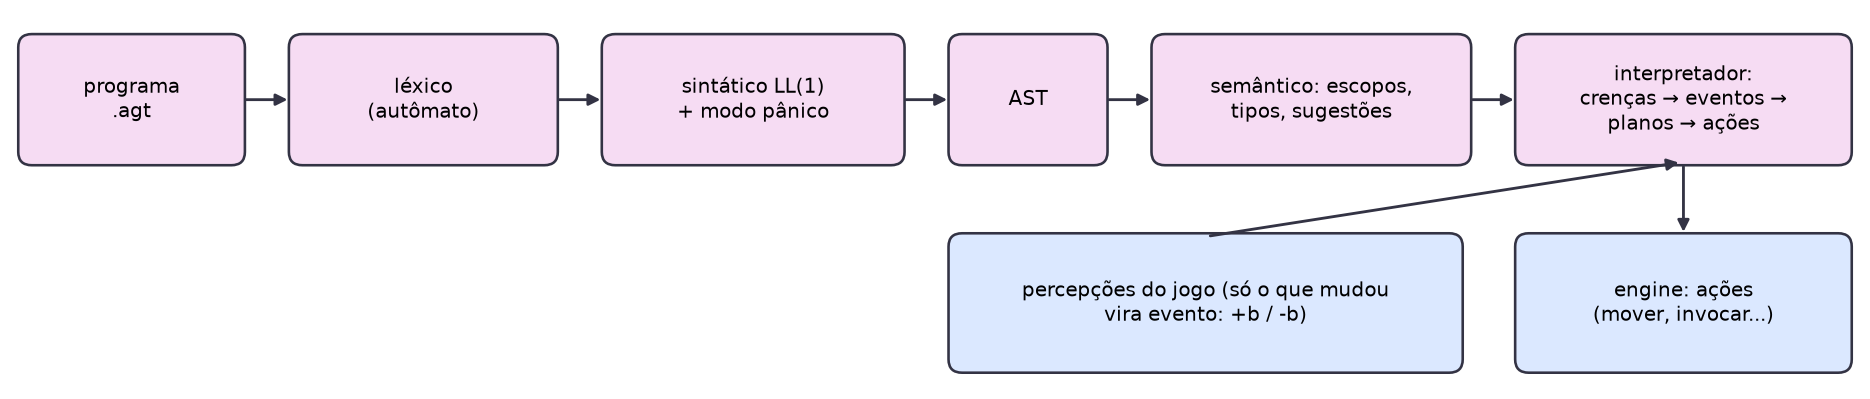
\includegraphics[width=\columnwidth]{figuras/dsl_pipeline.png}}
\caption{Fluxo do processador da AgentDSL, do código-fonte às ações na engine.}
\label{fig:arquitetura}
\end{figure}

\subsection{Gramática}
A gramática, em EBNF, é LL(1). Os principais não terminais são:
\begin{lstlisting}
programa  = { agente } ;
agente    = ("agente" | "modelo") IDENT [":" IDENT]
            "{" { crenca | plano } "}" ;
crenca    = literal "." ;
plano     = evento [":" contexto] "<-" corpo "." ;
evento    = ("+" | "-") ["!"] literal ;
contexto  = condicao { "&" condicao } ;
condicao  = "nao" literal | literal | expr op_rel expr ;
corpo     = acao { ";" acao } ;
acao      = ("+" | "-" | "-+") literal | "!" literal
          | IDENT ["(" args ")"] ;
literal   = IDENT ["(" args ")"] ;
expr      = termo { ("+" | "-") termo } ;
termo     = fator { ("*" | "/" | "%") fator } ;
fator     = NUM | VAR | IDENT | TEXTO | "(" expr ")" | "-" fator ;
\end{lstlisting}
Além da proposta inicial, foram acrescentados: \texttt{modelo}, que declara um \textit{tipo} de agente do qual o jogo cria várias instâncias (cada inimigo é uma instância); herança (\texttt{modelo chefe : inimigo}); variáveis, aritmética e comparações; negação (\texttt{nao}); \texttt{-+}, que substitui uma crença; e objetivos no estilo do Jason (\texttt{+!g}, \texttt{!g} e \texttt{-!g}).

\subsection{Análise Léxica}
O léxico funciona como um autômato: o primeiro caractere escolhe o estado (identificador, variável, número, texto ou símbolo) e o lexema cresce enquanto o próximo caractere for válido. Símbolos de dois caracteres, como \texttt{<-} e \texttt{<=}, têm prioridade (maior lexema). Cada token guarda linha e coluna. Caracteres inválidos, números malformados e textos não fechados geram erro léxico, e a análise continua.

\subsection{Análise Sintática}
O parser é descendente recursivo, com uma função por não terminal, e constrói a AST. Ao encontrar um erro, registra o que era esperado e entra em \textit{modo pânico}: descarta tokens até um ponto de sincronização (\texttt{.}, \texttt{\}} ou o início de outro agente). Assim, vários erros são relatados numa única execução.

\subsection{Análise Semântica}
O analisador mantém uma tabela de símbolos com três escopos: global (agentes e modelos), agente (assinaturas das crenças) e plano (variáveis). Ele verifica:
\begin{itemize}
\item nomes repetidos e herança de modelos inexistentes;
\item crenças iniciais com variáveis;
\item variáveis usadas sem estarem ligadas no evento ou no contexto (variáveis anônimas \texttt{\_X} são livres na negação);
\item ações desconhecidas, com sugestão do nome mais parecido;
\item número e tipo dos argumentos das ações (número, átomo, texto, modelo, crença);
\item aritmética com valores não numéricos;
\item objetivos \texttt{!g} sem nenhum plano \texttt{+!g}.
\end{itemize}
Também emite avisos, como um plano \texttt{-!g} sem o \texttt{+!g} correspondente ou um evento que nunca ocorrerá.

\subsection{Interpretador e Integração com a Engine}
Cada agente tem uma base de crenças e uma fila de eventos. Para cada evento, os planos com o mesmo gatilho são testados na ordem do código; o primeiro cujo gatilho \textit{unifica} e cujo contexto é satisfeito é executado. As ações de crença geram novos eventos; as demais são enviadas à engine. Quando um objetivo falha, a falha sobe até o objetivo mais interno que tenha um plano \texttt{-!g}, como no Jason, e a execução continua depois dele.
Na engine, o componente \textit{ServicoAgentes} compila o arquivo \texttt{.agt} e roda o ciclo de raciocínio a cada quadro, depois que os scripts geraram as percepções; cada objeto controlado recebe um componente \textit{ComportamentoAgente}. Cada jogo acrescenta ações e percepções escritas em Python, com assinatura:
\begin{lstlisting}
@acao_dsl("leque", "num", "num", "num")
def leque(corpo, agente, n, abertura, vel):
    ...   # cria n tiros abertos em leque
\end{lstlisting}
A partir daí, \texttt{leque(5, 70, 210)} passa a ser conferida pelo analisador semântico como as ações nativas. No editor da engine é possível criar e verificar arquivos \texttt{.agt}, e os erros aparecem no console com linha e coluna.

\section{Resultados e Discussão}
A linguagem foi usada em seis projetos de jogo. No \textit{shoot 'em up}, a IA dos inimigos, do chefe e do diretor das ondas está na DSL; o chefe muda de ataque conforme a vida cai:
\begin{lstlisting}
modelo inimigo {
    vida(1).  pontos(100).  item(6).
    +atingido(D) : vida(V) & V > D <- -+vida(V - D); piscar.
    +atingido(_D) : item(C) <- soltar_item(C); explodir.
}
modelo chefe : inimigo {
    vida(90). fase(1). nasceu.
    +nasceu <- ir_para(450, 470, 70).
    +ataque : fase(1) <- -ataque; leque(5, 70, 210);
                         temporizador(1.3, ataque).
    +vida(V) : fase(1) & V < 60 <- -+fase(2);
                         avisar("O chefe ficou bravo!").
}
\end{lstlisting}
No jogo de plataforma Fig.~\ref{fig:plataforma}, o slime vira ao perceber parede ou buraco à frente (eventos \texttt{+parede\_a\_frente} e \texttt{+buraco\_a\_frente}, gerados por consultas de raio da física), o caracol se esconde na concha no primeiro pisão, e até os blocos ``?'' são agentes que decidem o que soltar quando são batidos por baixo. Num jogo de programação, o próprio jogador escreve AgentDSL para controlar robôs, usando objetivos e planos de falha (\texttt{-!produzir <- jogar\_fora; !produzir.}).
\begin{figure}[htbp]
\centerline{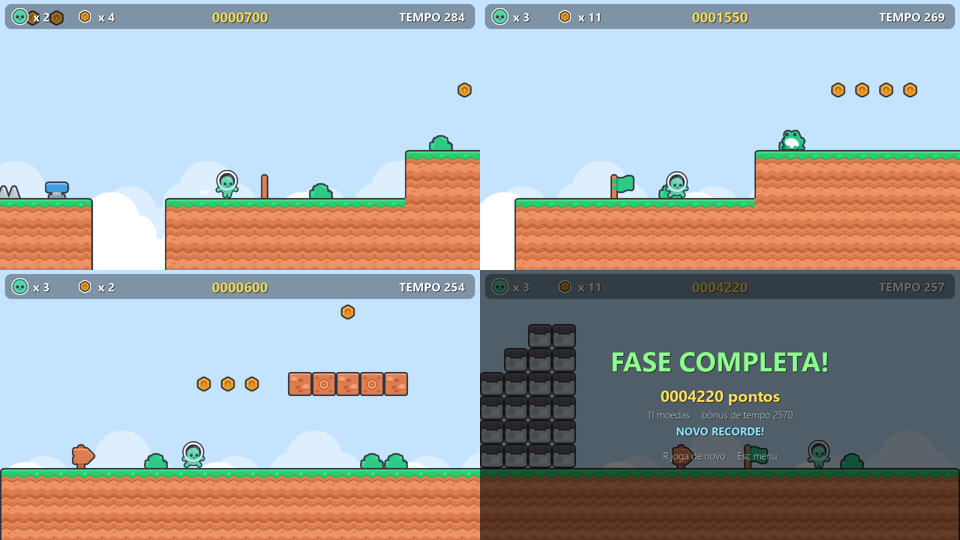
\includegraphics[width=\columnwidth]{figuras/plataforma_partida.png}}
\caption{Jogo de plataforma cujos inimigos e blocos são agentes escritos na DSL.}
\label{fig:plataforma}
\end{figure}
Para validar o compilador foram escritos programas com erros. Exemplos de mensagens produzidas:
\begin{lstlisting}
3:20: erro lexico: texto não fechado (faltou ")
5:20: erro sintatico: esperava '<-' entre o
      evento/contexto e as ações, encontrou 'velocidade'
8:14: erro semantico: ação desconhecida 'velocidad'
      (quis dizer 'velocidade'?)
11:20: erro semantico: variável 'Y' usada em 'mover'
       sem estar ligada no evento ou no contexto
\end{lstlisting}
Para avaliar se a DSL simplifica a tarefa, o comportamento de dois inimigos foi reescrito em Python (Tabela~\ref{tab:concisao}). A versão em Python precisa guardar o valor anterior de cada percepção e controlar temporizadores manualmente, o que a DSL faz pelos eventos.
\begin{table}[htbp]
\caption{Mesmo comportamento (dois inimigos) nas duas linguagens}
\begin{center}
\begin{tabular}{lrr}
\toprule
Versão & Linhas & Tokens \\
\midrule
AgentDSL & 23 & 217 \\
Python & 61 & 382 \\
\bottomrule
\end{tabular}
\label{tab:concisao}
\end{center}
\end{table}
Em desempenho (Tabela~\ref{tab:desempenho}), um programa com 1 000 agentes (116 mil tokens) passou pelas três análises em cerca de 1 segundo, e o interpretador processou entre 178 e 217 mil eventos por segundo, o suficiente para centenas de agentes a 60 quadros por segundo. O projeto tem 110 testes automáticos, que cobrem as quatro fases e os jogos jogados até o fim por um robô.
\begin{table}[htbp]
\caption{Desempenho do processador da linguagem}
\begin{center}
\begin{tabular}{lr}
\toprule
Medida & Resultado \\
\midrule
Léxico (1 000 agentes) & 707 ms \\
Sintático & 175 ms \\
Semântico & 81 ms \\
Interpretador (10 agentes) & 217 mil eventos/s \\
Interpretador (1 000 agentes) & 178 mil eventos/s \\
\bottomrule
\end{tabular}
\label{tab:desempenho}
\end{center}
\end{table}

\section{Conclusão}
Foi desenvolvida uma DSL orientada a eventos para controlar agentes de uma engine 2D, com análise léxica, sintática e semântica e um interpretador integrado à engine e ao seu editor. A linguagem permitiu descrever inimigos, chefes, torres, blocos e ondas de seis jogos com regras curtas, separando o comportamento da parte gráfica, e os objetivos com tratamento de falhas aproximaram o modelo do Jason.
Os principais desafios foram a recuperação de erros no parser, a verificação de tipos com variáveis e a integração com o loop da engine, resolvida fazendo os agentes reagirem depois que as percepções do quadro são geradas. Como expansões, propõem-se comunicação entre agentes no estilo das mensagens do Jason, compilação dos planos para \textit{bytecode} e realce de sintaxe para editores de código.

\begin{thebibliography}{00}
\bibitem{mernik2005} M. Mernik, J. Heering and A. M. Sloane, ``When and how to develop domain-specific languages,'' \textit{ACM Computing Surveys}, vol. 37, no. 4, pp. 316--344, 2005.
\bibitem{vandeursen2000} A. van Deursen, P. Klint and J. Visser, ``Domain-specific languages: An annotated bibliography,'' \textit{ACM SIGPLAN Notices}, vol. 35, no. 6, pp. 26--36, 2000.
\bibitem{rodrigues2017} I. P. Rodrigues, M. B. Campos and A. F. Zorzo, ``Usability evaluation of domain-specific languages: a systematic literature review,'' in \textit{Human-Computer Interaction (HCI International)}, 2017.
\bibitem{rao1996} A. S. Rao, ``AgentSpeak(L): BDI agents speak out in a logical computable language,'' in \textit{Agents Breaking Away (MAAMAW)}, LNCS 1038, Springer, 1996, pp. 42--55.
\bibitem{rao1995} A. S. Rao and M. P. Georgeff, ``BDI agents: From theory to practice,'' in \textit{Proc. 1st Int. Conf. on Multi-Agent Systems (ICMAS)}, 1995, pp. 312--319.
\bibitem{bordini2007} R. H. Bordini, J. F. Hübner and M. Wooldridge, \textit{Programming Multi-Agent Systems in AgentSpeak using Jason}. Chichester: Wiley, 2007.
\bibitem{aho2006} A. V. Aho, M. S. Lam, R. Sethi and J. D. Ullman, \textit{Compilers: Principles, Techniques, and Tools}, 2nd ed. Boston: Addison-Wesley, 2006.
\bibitem{hopcroft2006} J. E. Hopcroft, R. Motwani and J. D. Ullman, \textit{Introduction to Automata Theory, Languages, and Computation}, 3rd ed. Boston: Addison-Wesley, 2006.
\end{thebibliography}

\end{document}
